% Created 2021-01-24 Sun 22:49
% Intended LaTeX compiler: pdflatex
\documentclass[11pt]{article}
\usepackage[utf8]{inputenc}
\usepackage[T1]{fontenc}
\usepackage{graphicx}
\usepackage{grffile}
\usepackage{longtable}
\usepackage{wrapfig}
\usepackage{rotating}
\usepackage[normalem]{ulem}
\usepackage{amsmath}
\usepackage{textcomp}
\usepackage{amssymb}
\usepackage{capt-of}
\usepackage{hyperref}
\usepackage{minted}
\hypersetup{colorlinks=true, linkcolor=black, filecolor=red, urlcolor=blue}
\usepackage[turkish]{babel}
\author{Eren Hatırnaz}
\date{13 Nisan 2020}
\title{Yazılım Gündemi - 2020/14\\\medskip
\large 6-12 Nisan 2020}
\hypersetup{
 pdfauthor={Eren Hatırnaz},
 pdftitle={Yazılım Gündemi - 2020/14},
 pdfkeywords={},
 pdfsubject={},
 pdfcreator={Emacs 27.1 (Org mode 9.3)},
 pdflang={Turkish}}
\begin{document}

\maketitle
\tableofcontents \clearpage\shorthandoff{=}

\begin{center}
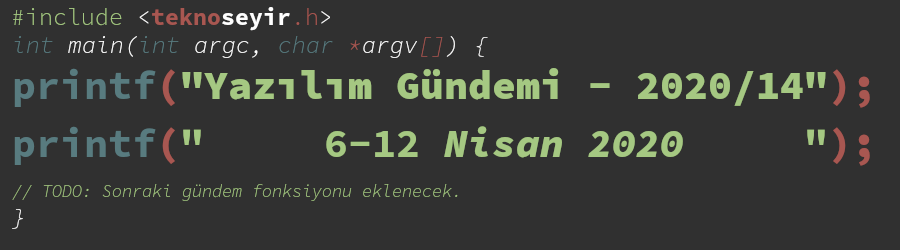
\includegraphics[width=.9\linewidth]{gorseller/yazilim-gundemi-banner.png}
\end{center}

\begin{center}
\href{../13/yazilim-gundemi-2020-13.pdf}{< Önceki Gündem} | \textbf{6-12 Nisan 2020} | \href{../15/yazilim-gundemi-2020-15.pdf}{Sonraki Gündem >}

\href{https://teknoseyir.com/blog/yazilim-gundemi-2020-14}{TeknoSeyir'de Oku}
\end{center}

\section{Qt, \href{https://www.qt.io/blog/qt-roadmap-for-2020}{2020 yılı için bir yol haritası} yayınladı fakat \href{https://www.phoronix.com/scan.php?page=news\_item\&px=Qt-Might-Restrict-New-Releases}{söylenmeyenler olabilir}}
\label{sec:org4ae9a49}
C++ dünyasının popüler platformlar-arası (cross-platform) uygulama geliştirme
framework'lerinden biri olan Qt, bu hafta içerisinde 2020 yılı yol haritasını
yayınladı fakat KDE projesinin açık e-posta listesindeki bazı ifadeler 2020
yılı planının söylenmeyen bazı kısımlarını açığa çıkardı. Öncelikle Qt'nin
blog yazısı ile birlikte duyurduğu yol haritasına bakalım.

\begin{itemize}
\item Qt Design Studio 1.5 sürümü Mayıs ayı içerisinde yayınlanacak.
\begin{itemize}
\item Bu sürümde 2 boyutlu ve 3 boyutlu tasarımla ilgili iyileştirilmeler
yapılmış, bu konularda çalışmaya devam edeceklermiş.
\item Annotations desteği: Uygulamanın tasarımı ve geliştirilmesi devam ederken
sadece geliştiricilerin görebileceği notlar bırakabileceğiz. Bir nevi
tasarım ekranındaki yorum satırları diyebiliriz.
\item Adobe XD vb. diğer araçlar için destek çalışmaları devam ediyormuş.
\end{itemize}
\item Qt Creator aracına C++20 desteği ekleniyor.
\begin{itemize}
\item Python ve QML desteklerini iyileştirmek için çalışmalar devam ediyor.
\end{itemize}
\item CMake 3.17 desteği gelecek.
\item Qt 5.15 ile birlikte yeni bir Qt for Microcontrollers sürümü de gelecek ve
tam QML desteği sağlayacak. Qt for MCUs için araçlar üzerinde çalışılıyor.
Qt Design Studio yazılımına MCU desteği gelecek.
\item Qt 1.15 sürümü Mayıs ayının sün günlerinde yayınlanacak. Ticari kullanım
lisansı olanlar için LTS (Long-term support/Uzun-dönemli destek) olacak
fakat açık kaynak kullanıcılar için normal bir sürüm olarak gelecek.
\begin{itemize}
\item Qt Quick 3D desteğiyle gelecek.
\item Metal ve Vulkan gibi grafik API'lerini kullanabilmek için yeni Rendering
Hardware Interface gelecek.
\end{itemize}
\item Qt'nin bir sonraki büyük sürümü Qt 6.0'ın bu yılın sonunda yayınlanması
planlanıyor.
\item Qt'nin araç setindeki yazılımlara Qt Marketplace entegrasyonu eklemek için
çalışmalar devam ediyor.
\end{itemize}

Diğer detayları okumak isterseniz Qt firmasının blog sitesideki \href{https://www.qt.io/blog/qt-roadmap-for-2020}{şu yazıya}
bakabilirsiniz. \href{https://www.phoronix.com/scan.php?page=news\_item\&px=Qt-2020-Roadmap}{Alternatif}

Şimdi gelelim asıl meseleye. Bu yılın ilk yazılım gündemi yazılarının birinde
(bkz: \href{../05/yazilim-gundemi-2020-05.pdf}{Yazılım Gündemi - 2020/05}), Qt'nin 2020 yılına değişikliklerle girdiğini
ve bunlar arasında da LTS sürümlerinin sadece ücretli lisans kullanıcılarına
sunulacağı vardı. Fakat Qt firmasının yukarıdaki yol haritasının yayınlandığı
gün, KDE projesinin e-posta listesinden tüm KDE topluluğuna "\emph{Qt, Open Source
and corona}" başlıklı bir e-posta da gönderildi. E-posta'da Qt ve KDE
projeleri arasındaki bir takım tarihsel bilgilerden sonra geçtiğimiz hafta Qt
firmasının KDE takımlarıyla ile iletişime geçerek, "koronavirüs salgınının yol
açacağı ekonomik sorunlar yüzünden yeni yayınlanacak tüm Qt sürümlerinin 12 ay
süresince sadece ücretli lisans sahiplerine sunmayı" düşündüklerini iddia eden
ifadeler yer aldı. Bunun üzerine 9 Nisan tarihinde \href{https://www.qt.io/blog/qt-and-open-source}{bir yazı daha yayınlayarak}
ilgili bilgilerin, "Qt firmasının plan ve görüşlerini yansıtmadığını"
söylediler. Konu tabii ki \href{https://www.reddit.com/r/cpp/comments/fxbo24/qt\_open\_source\_and\_corona/}{Reddit} gibi platformlarda tartışmalara yol açtı.

C++ ve Qt ekosistemine uzak birisi olarak bu haberi doğru
yorumlayamayabilirim. O yüzden aramızdaki bu alanlarda çalışmış kişilerden
görüşlerini yorumlar bölümünde belirtmelerini rica ediyorum. Qt'nin gerçekten
böyle bir karar verip vermediği ilerleyen haftalarda ortaya çıkacak fakat
böyle bir kararın açık kaynak topluluklarına bölünmelere yol açacağı ortada.
Umarım Qt firması kararlarını tekrar gözden geçirir.
\section{Firefox 75.0 ile \href{https://hacks.mozilla.org/2020/04/firefox-75-ambitions-for-april/}{gelen yeni özellikler}}
\label{sec:orgddc0d88}
Mozilla tarafından geliştirilen Firefox tarayıcısının 75.0 numaralı sürümü bu
hafta içerisinde yayınlandı. Peki bu yeni sürümle birlikte biz geliştiricileri
ilgilendiren neler var? Gelin birkaç tanesini birlikte inceleyelim.

\subsection{Tembel resim yükleme (lazy-loading)}
\label{sec:orge3d96fa}
Geçtiğimiz yazılım gündemi yazılarından birinde (bkz: \href{../07/yazilim-gundemi-2020-07.pdf}{Yazılım Gündemi -
2020/07}) bu özelliğin W3C tarafından onaylanmış bir internet standardı
olduğunu duyurmuştum. İşte o özellik bu hafta Firefox'a da geldi. O yazıyı
okumayanlar için kısaca özetlemek gerekirse: artık aşağıdaki gibi etiketlenmiş
bir görsel sayfa açıldığında hemen yüklenmeyecek, sadece ekranda görünür
olduğunda yüklenecek.

\begin{minted}[breaklines=true,breakanywhere=true,frame=lines, linenos, label=HTML]{html}
<img src="teknoseyir.png" loading="lazy" alt="TeknoSeyir Logo" />
\end{minted}
Bu sayede web sayfalarımız hem bize hem de kullanıcılara gereksiz trafik yükü
oluşturmayacak.

Bu özelliği destekleyen tarayıcılar ise şu şekilde:

\begin{figure}[htbp]
\centering
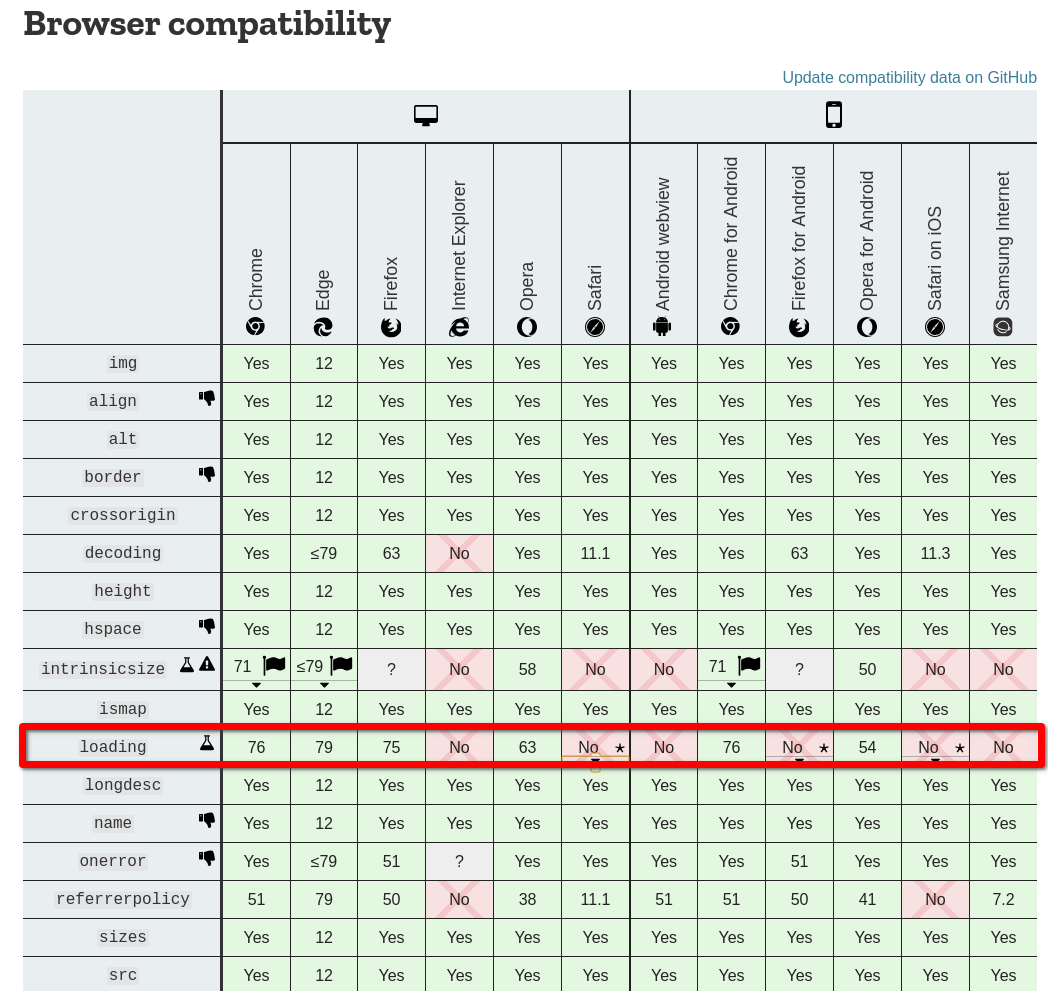
\includegraphics[width=.9\linewidth]{gorseller/lazy-loading-uyumluluk.png}
\caption[//developer.mozilla.org/en-US/docs/Web/HTML/Element/img\#Browser\_compatibility]{Kaynak: Mozilla Developer Network - \url{https://developer.mozilla.org/en-US/docs/Web/HTML/Element/img\#Browser\_compatibility}}
\end{figure}
\newpage

Lazy loading özelliği hakkında daha fazla bilgi almak için \href{https://developer.mozilla.org/en-US/docs/Web/Performance/Lazy\_loading}{buraya}
tıklayabilirsiniz.
\subsection{Konsolda çoklu-satır modu ve anında sonuç görme}
\label{sec:orgca2cbaa}
JavaScript ile web geliştirme yapanlarımızın adeta eli ayağı gibi olan
Developer Tools aracının Console kısmında artık çok-satırlı kod yazıp
çalıştırabileceğiz. Bu özelliği açmak için Console sekmesindeyken \textbf{CTRL+B}
tuşlarına basmanız yeterli.

\begin{center}
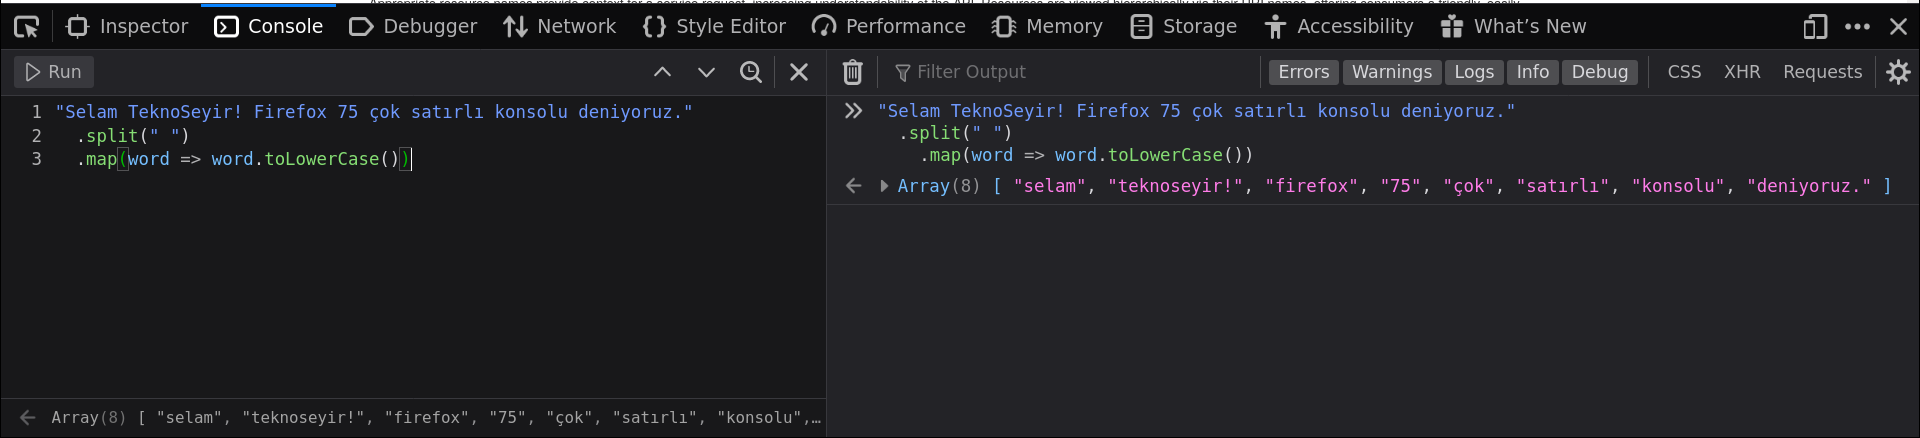
\includegraphics[width=.9\linewidth]{gorseller/firefox75-console.png}
\end{center}

Çoklu satır modu açıldığında kodlarınızı yazdığınız yerin yanına bir panel
daha açılacak. Bu panel kodlarınızı çalıştırdıktan sonra sonuçlarını
göreceğiniz ekran. Artık çoklu satır modunda olduğunuz için \textbf{ENTER} ile
kodlarınızı çalıştıramayacaksınız, bunun yerine \textbf{CTRL+ENTER} kullanmanız
gerekiyor. Ayrıca burada yazdığınız kodları bir dosyaya kaydetmek
istiyorsanız da \textbf{CTRL+S} tuş kombinasyonlarını kullanabilirsiniz. Çok-satır
modu hakkında daha fazla bilgi için \href{https://developer.mozilla.org/en-US/docs/Tools/Web\_Console/The\_command\_line\_interpreter\#Multi-line\_mode}{buraya} tıklayabilirsiniz.

Yukarıdaki ekran görüntüsünün en altında bir de \texttt{Array(8)} ile başlayan bir
satır görüyorsunuz. O ise bu sürümle birlikte gelen "\emph{Instant Evaluation}"
özelliği. Biz kodumuzu yazdıkça orası anlık olarak güncelleniyor ve
yazdığımız kodun sonucunu bize ön-izleme olarak sunuyor. Gayet güzel ve
faydalı bir özellik.
\subsection{CSS için \texttt{min()}, \texttt{max()}, \texttt{clamp()} fonksiyonları}
\label{sec:orgd7d6f9d}
Bu fonksiyonlar ile artık css tarafında bazı hesaplamalar yapabileceğiz.
Şöyle ki:

\begin{itemize}
\item \href{https://developer.mozilla.org/en-US/docs/Web/CSS/min}{min()}: Bir ya da daha fazla değer alır ve bunlar içerisinden \textbf{en küçük}
olanı döndürür.
\item \href{https://developer.mozilla.org/en-US/docs/Web/CSS/max}{max()}: Bir ya da daha fazla değer alır ve bunlar içerisinden \textbf{en büyük}
olanı döndürür.
\item \href{https://developer.mozilla.org/en-US/docs/Web/CSS/clamp}{clamp()}: \texttt{minimum}, \texttt{tercih edilen} ve \texttt{maximum} olmak üzere üç değer
alır. Eğer hesaplanan değer minumum'dan küçükse \texttt{minimum}; maximum'dan
büyükse \texttt{maximum} değer geçerli olur. Eğer hesaplanan değer ikisinin
arasındaysa \texttt{tercih edilen} değer geçerli olur.

Tahmin edebileceğiniz gibi bu fonksiyonların hepsi responsive tasarım için
düşünülmüş ve eklenmiş özellikler. Böylece web sitelerimizin tasarımlarında
daha özel hesaplamalar yapabileceğiz. Fonksiyonlar hakkında detaylar ve
tarayıcı uyumluluğu listesi için her fonksiyonun kendi bağlantısına
tıklayabilirsiniz.
\end{itemize}

Firefox'un bu sürümüyle birlikte gelen diğer özellikler için konu başlığına
eklediğim bağlantıya tıklayabilirsiniz.
\section{IntelliJ IDEA \href{https://blog.jetbrains.com/idea/2020/04/intellij-idea-2020-1-released/}{2020.1 sürümü yayınlandı}}
\label{sec:org35f0c96}
JetBrains tarafından geliştirilen ve topluluk için ücretsiz sürümü de bulunan,
Java için geliştirme ortamı (IDE) olan IntelliJ IDEA'nın 2020 yılındaki ilk
sürümü olan 2020.1, bu hafta içerisinde yayınlandı. Bu sürümle birlikte gelen
birkaç özellik şu şekilde:

\begin{itemize}
\item Java 14 desteği,
\item Artık JDK'yı direkt IDE'nin içerisinden indirip kullanabileceksiniz,
\item LightEdit Modu (detaylar aşağıda),
\item Zen Modu: Distraction Free Mode (Sıfır dikkat dağınıklığı modu) ve tam
ekran modunu bir araya getiren, odaklı bir şekilde kod yazmayı vaad eden
bir mod.
\item Varsayılan yazı tipi \href{http://jetbrains.com/lp/mono/}{JetBrains Mono} olarak değiştirildi,
\end{itemize}

\subsection{\href{https://blog.jetbrains.com/idea/2020/04/lightedit-mode/}{Light Edit Mode}}
\label{sec:org2a725d8}
\begin{center}
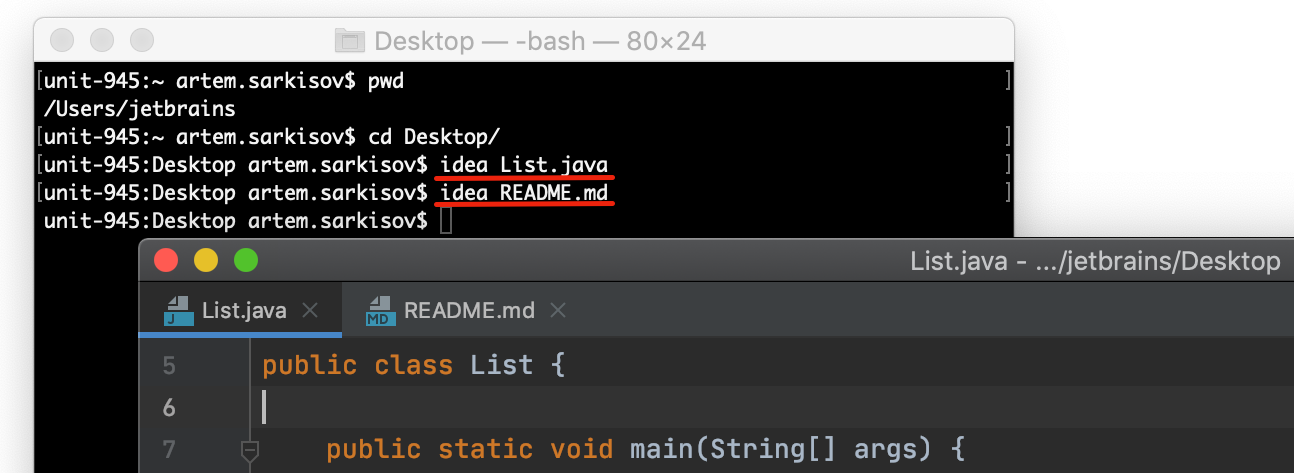
\includegraphics[width=.9\linewidth]{gorseller/intellij-idea-lightedit-terminal.png}
\end{center}

Yazılım Gündemi yazılarını düzenli olarak takip edenler böyle bir özelliğin
geleceğinden haberdardı :) (bkz: \href{../04/yazilim-gundemi-2020-04.pdf}{Yazılım Gündemi - 2020/04}) Haberdar olmayan
yeni takipçiler için açıklayalım: JetBrains'in IDE'lerini en az bir kez
kullanmışsanız biliyorsunuzdur ki, IDE'nin açılması ve projeyle ilgili
cache'leme işlemlerinin yapılması çok uzun sürüyordu. Artık terminal'den
sadece dosya ismiyle IntelliJ IDEA'yı çağırdığınızda IDE Light Edit modunda
açılıyor ve gelişmiş bir metin editörü gibi davranarak sadece o dosyayı
açıyor. Proje'nin geri alanını yüklemiyor.

\begin{figure}[htbp]
\centering
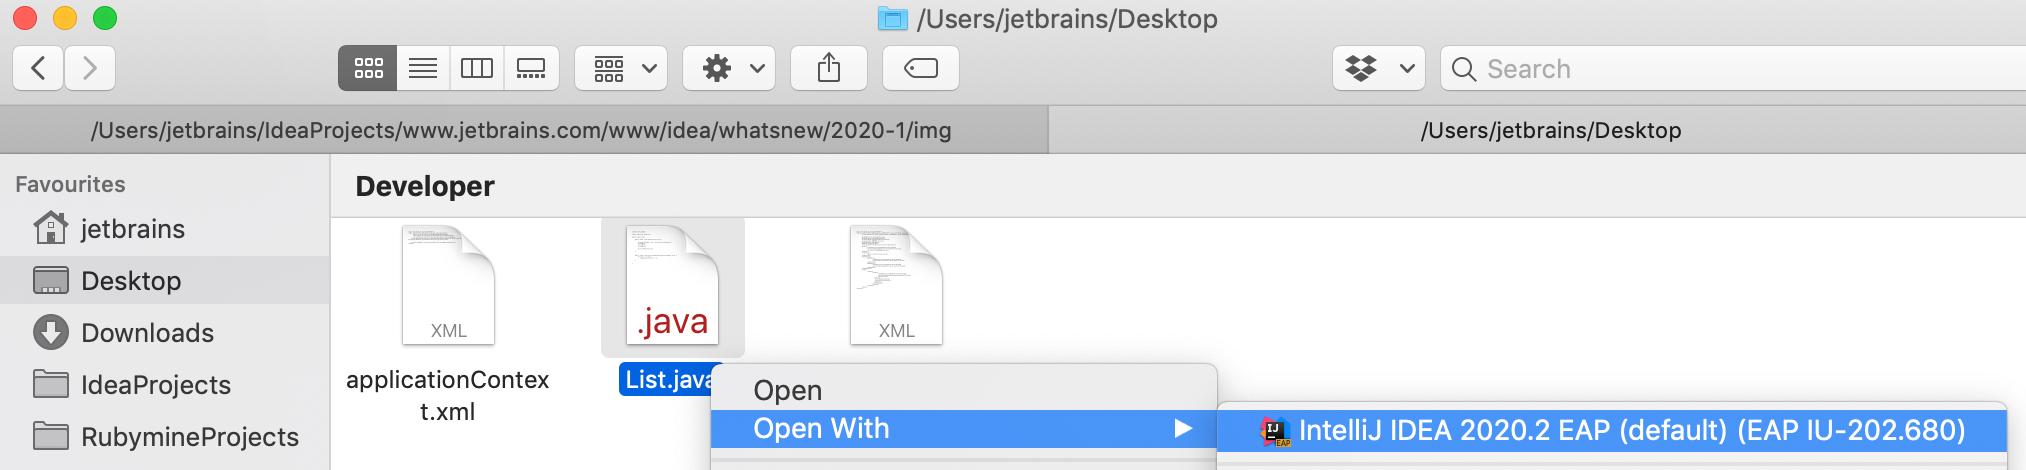
\includegraphics[width=.9\linewidth]{gorseller/intellij-idea-lightedit-sag-tik.png}
\caption{Light Edit modunu terminal ekranından açmak zorunda değilsiniz. Sağ tık menüsünden "Birlikte Aç" ile de açabilirsiniz.}
\end{figure}

Yalnız bir istisna var: Eğer açmak istediğiniz dosyanın bağlı olduğu proje
zaten normal modda Intellij IDEA üzerinde açıkca, LightEdit modu açılmaz, var
olan proje penceresine yeni bir sekme olarak gelir.

\begin{figure}[htbp]
\centering
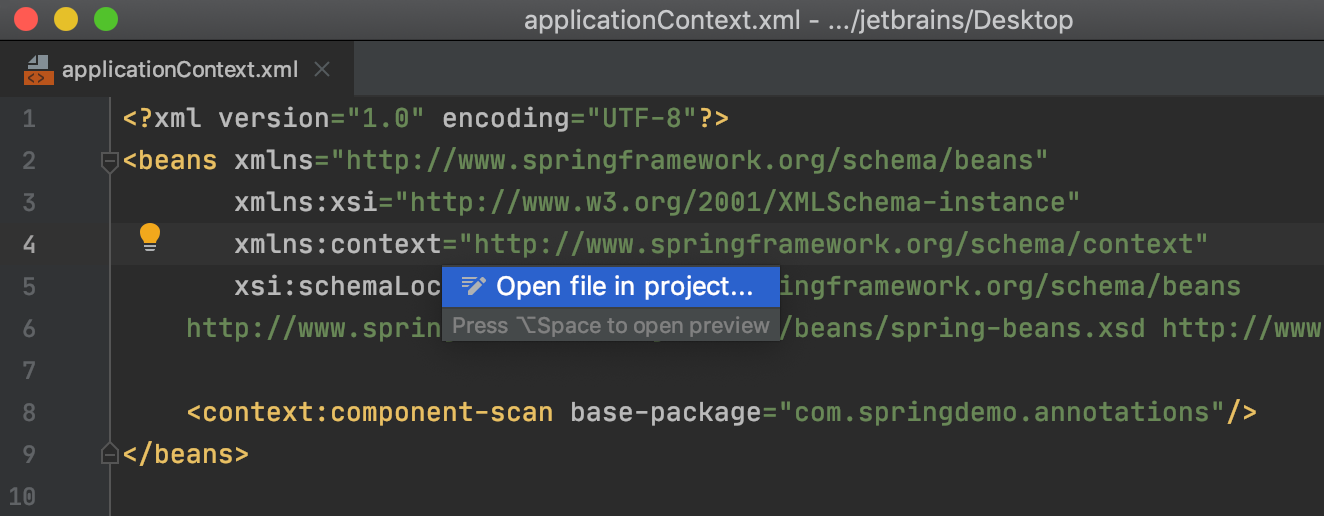
\includegraphics[width=.9\linewidth]{gorseller/intellij-idea-light-editproject-mode.png}
\caption{Tekrar normal proje moduna geçmek için File menüsü içerisinden ya da \textbf{ALT+ENTER} ile açılan menüden "Open File in Project" seçeneğini seçebilirsiniz.}
\end{figure}
\newpage
Intellij IDEA'nın bu sürümüyle birlikte gelen diğer özellikler için aşağıdaki
videoyu izleyebilir ya da konu başlığına eklediğim bağlantıya
tıklayabilirsiniz. Aynı şekilde Light Edit modunun detayları için de alt konu
başlığına tıklayabilirsiniz.

\begin{itemize}
\item \href{https://www.youtube.com/watch?v=LtOH7snHBCA}{Konuyla ilgili YouTube videosu}
\newpage
\end{itemize}
\section{Google SRE \href{https://security.googleblog.com/2020/04/introducing-our-new-book-building.html?m=1}{yeni kitap tanıttı}: "\href{https://landing.google.com/sre/books/}{Building Secure and Reliable Systems}"}
\label{sec:orgd1d60de}
\begin{center}
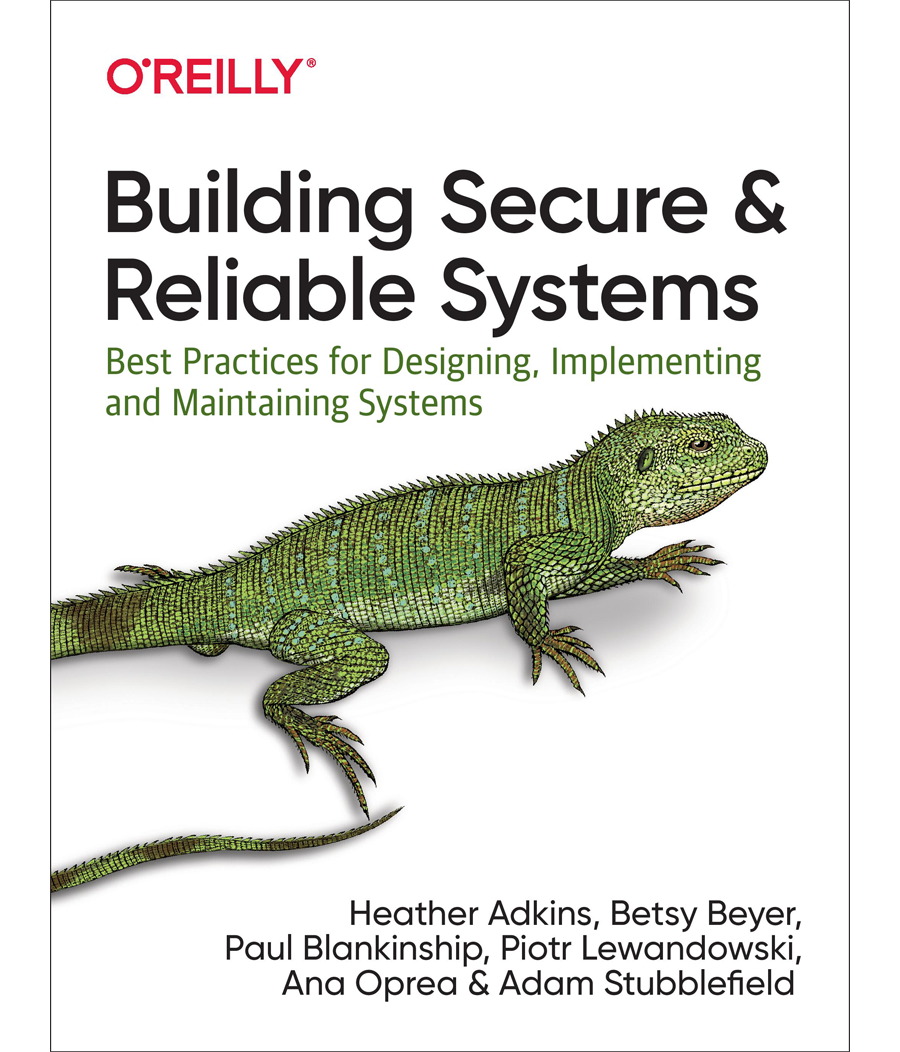
\includegraphics[height=5cm]{gorseller/google-kitap.png}
\end{center}

Google'ın Site Reliability Engineering (SRE) projesi kapsamında çıkan 3.kitabı
raflarda ve \href{https://www.google.com/books/edition/Building\_Secure\_and\_Reliable\_Systems/Kn7UxwEACAAJ}{çevrim içi mağaza}larda yerini aldı. Google kitabı dijital kopyasını
çeşitli formatlarda kendi sitesi üzerinden de dağıtıyor.
\begin{itemize}
\item PDF formatında indirmek için: \url{https://landing.google.com/sre/static/pdf/SRS.pdf}
\item EPUB formatında indirmek için: \url{https://landing.google.com/sre/static/pdf/srs-epub.epub}
\item Mobi formatında indirmek için: \url{https://landing.google.com/sre/static/pdf/srs-mobi.mobi}
\end{itemize}
\section{Visual Studio Code \href{https://code.visualstudio.com/updates/v1\_44}{Mart 2020 (1.44) sürümü yayınlandı}}
\label{sec:orge7a960d}
\begin{center}
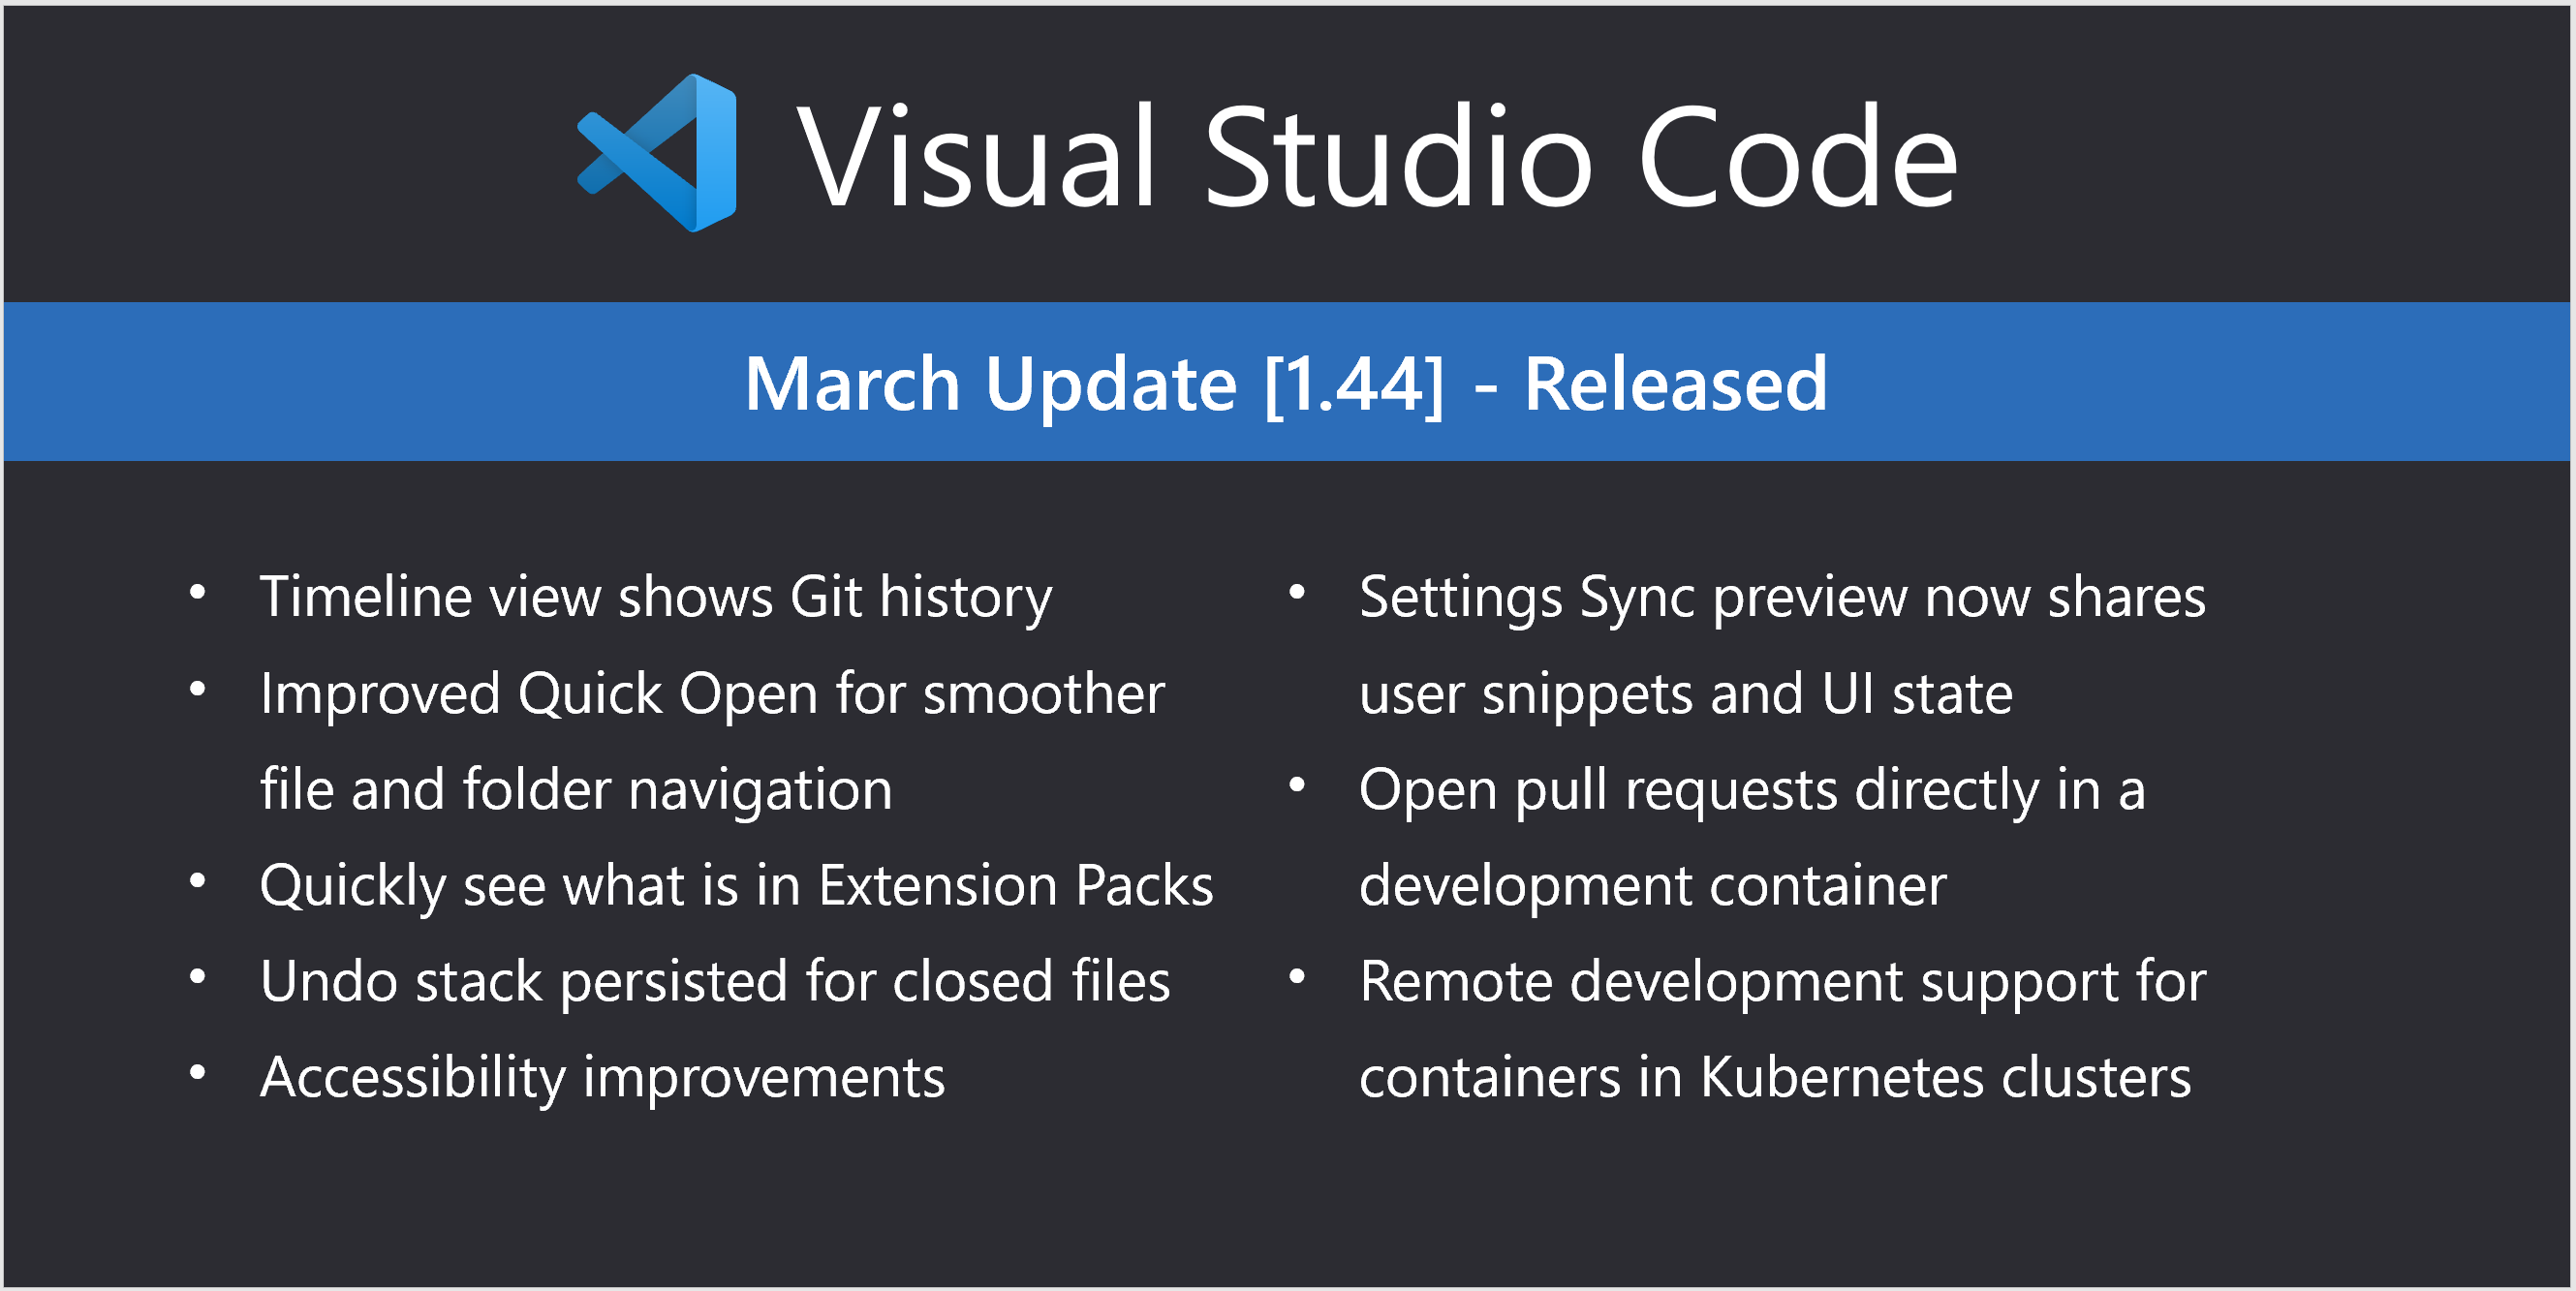
\includegraphics[width=.9\linewidth]{gorseller/vscode-144.png}
\end{center}
\section{Yaklaşan Etkinlik: "\href{http://www.acikseminer.com/}{Açık Seminerler (Türkiye Açık Kaynak Topluluğu)}"}
\label{sec:org14b5a1e}
\begin{center}
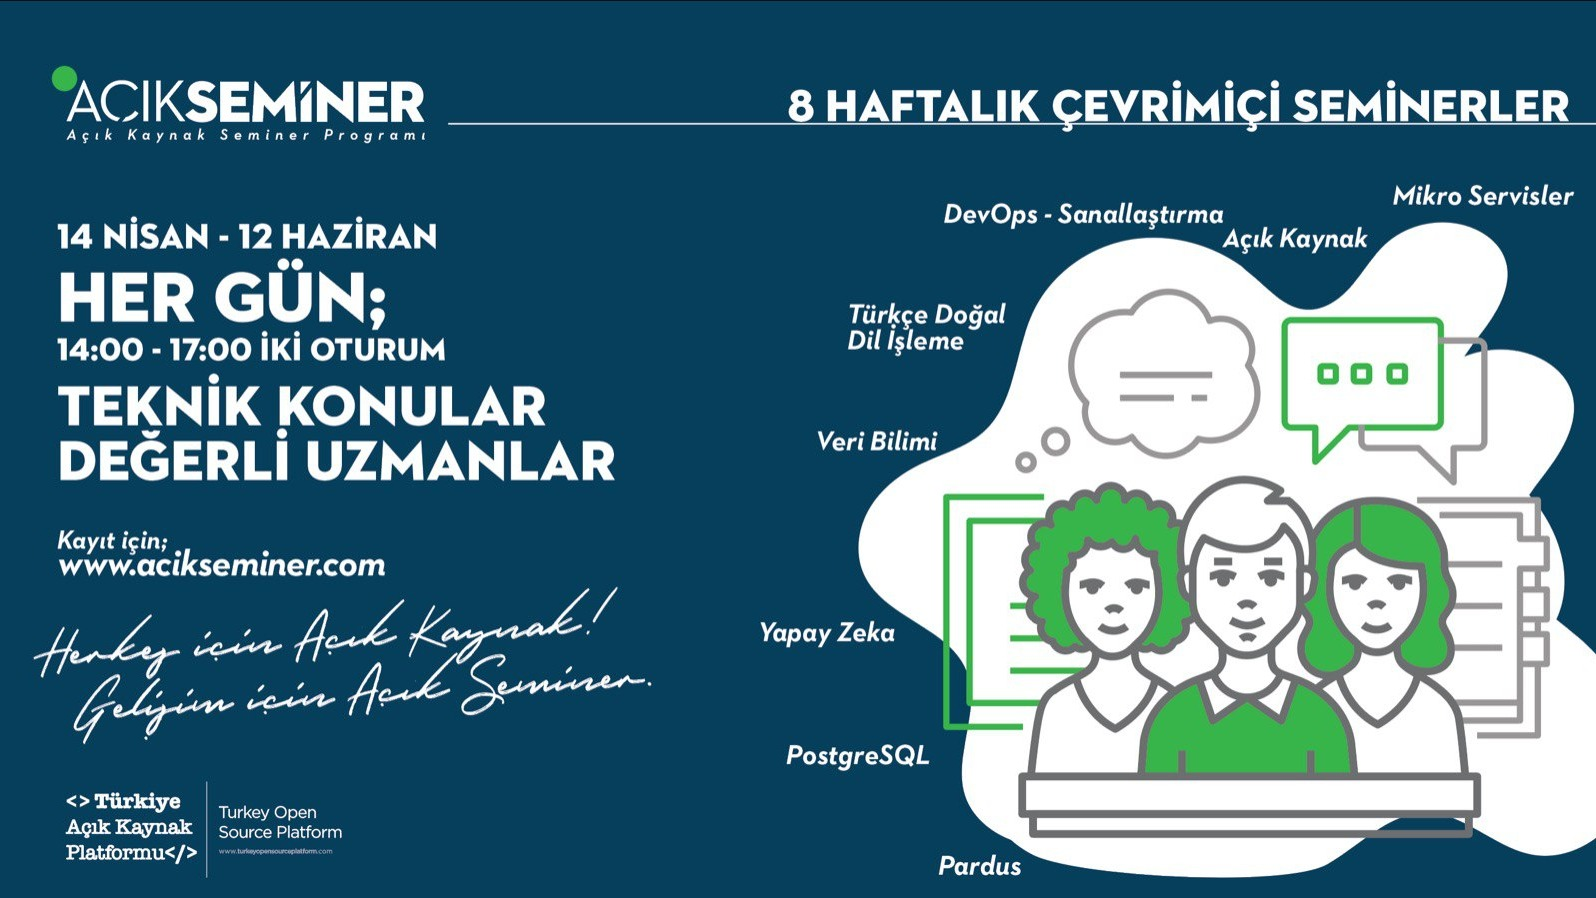
\includegraphics[width=.9\linewidth]{gorseller/acik-seminer.jpeg}
\end{center}
\newpage
\section{Diğer Haberler}
\label{sec:orge6cb317}
\begin{itemize}
\item Google ve Apple, Covid-19 takibi için \href{https://www.apple.com/newsroom/2020/04/apple-and-google-partner-on-covid-19-contact-tracing-technology/}{işbirliği yapmaya karar verdi}.
\href{https://www.bbc.com/news/technology-52246319}{Alternatif}
\item ABD'de Covid-19 yüzünden \href{https://nymag.com/intelligencer/2020/04/what-is-cobol-what-does-it-have-to-do-with-the-coronavirus.html}{COBOL programcıları göreve çağırıldı}.
\begin{itemize}
\item IBM, \href{https://www.inputmag.com/tech/ibm-will-offer-free-cobol-training-to-address-overloaded-unemployment-systems}{ücretsiz COBOL eğitimi} vermeyi teklif ediyor.
\end{itemize}
\item Git \href{https://opensource.com/article/20/4/get-started-git}{15 yaşında}! \href{https://github.blog/2020-04-07-celebrating-15-years-of-git-an-interview-with-git-maintainer-junio-hamano/}{Geliştirici takımından biriyle röportaj yazısı}.
\item Docker, Compose aracını geliştirmek için yeni bir \href{https://www.docker.com/blog/announcing-the-compose-specification/}{açık topluluk oluşturdu}:
\href{https://compose-spec.io/}{Compose Specification}. \href{https://github.com/compose-spec}{GitHub Organizasyon Sayfası}
\item Linux Vakfı, güvenlik odaklı kernel olan \href{https://sel4.systems/About/}{SeL4}'e \href{https://www.zdnet.com/article/linux-foundation-backs-security-oriented-sel4-microkernel-operating-system/}{destek oluyor}.
\item \href{https://www.mapzen.com/}{Mapzen} açık kaynaklı haritalama projesi artık Linux Vakfı altındaki \href{https://uc.foundation/}{Urban
Computing Foundation} projesi \href{https://www.zdnet.com/article/mapzen-open-source-mapping-project-revived-under-the-urban-computing-foundation/}{oldu}.
\item Amazon Elastic Container Service, artık Amazon EFS \href{https://aws.amazon.com/tr/blogs/aws/amazon-ecs-supports-efs/}{dosya sistemlerini
destekliyor}.
\item \href{https://www.sandboxie.com/}{Sandboxie} yıllar sonra \href{https://news.sophos.com/en-us/2020/04/09/sandboxie-is-now-an-open-source-tool/}{açık kaynak oldu}.
\item WebStorm \href{https://blog.jetbrains.com/webstorm/2020/04/webstorm-2020-1/}{2020.1 sürümü yayınlandı}.
\item NodeJS iki dalda yeni sürüm yayınladı:
\begin{itemize}
\item \href{https://nodejs.org/en/blog/release/v12.16.2/}{Node v12.16.2 (LTS)}
\item \href{https://nodejs.org/en/blog/release/v10.20.1/}{Node v10.20.1 (LTS)}
\end{itemize}
\item Go programlama dilinin \href{https://golang.org/doc/devel/release.html\#go1.14.minor}{1.41.2} ve \href{https://golang.org/doc/devel/release.html\#go1.13.minor}{1.13.10} \href{https://groups.google.com/forum/m/\#!msg/golang-announce/9UJN3gwMzhY/HVdQFNOVBgAJ}{sürümleri yayınlandı}.
\item Crystal programlama dilinin \href{https://crystal-lang.org/2020/04/06/crystal-0.34.0-released.html}{0.34.0 sürümü yayınlandı}.
\item \href{https://cuelang.org/}{Cue} programlama dilinin \href{https://github.com/cuelang/cue/releases/tag/v0.1.0}{v0.1.0 sürümü yayınlandı}.
\item ASP.NET Core için \href{https://ext.net/v7-0-preview-for-asp-net-core/}{Ext.NET 7.0 Preview yayınlandı}.
\item Kubernetes IDE'si Lens, \href{https://github.com/lensapp/lens/releases/tag/v3.2.0}{v3.2.0 sürümünü yayınladı}.
\item Apache Flink, Stateful Functions \href{https://flink.apache.org/news/2020/04/07/release-statefun-2.0.0.html}{2.0 sürümünü yayınladı}.
\item CheerpJ \href{https://medium.com/leaningtech/cheerpj-2-1-released-java-bytecode-to-webassembly-and-javascript-303fb8dd5d98}{2.1 sürümü yayınlandı}.
\item Spring Graal Native \href{https://spring.io/blog/2020/04/09/spring-graal-native-0-6-0-released}{0.6.0 sürümü yayınlandı}.
\item Horray \href{https://www.freerdp.com/2020/04/09/2\_0\_0-released}{2.0.0 sürümü yayınlandı}.
\item PyOxidizer \href{https://gregoryszorc.com/blog/2020/04/09/pyoxidizer-0.7/}{0.7 sürümü yayınlandı}.
\end{itemize}
\section{Lisans}
\label{sec:org2d97698}
\begin{center}
\begin{center}

\includegraphics[height=1.5cm]{../../../img/CC_BY-NC-SA_4.0.png}
\end{center}

\href{yazilim-gundemi-2020-14.pdf}{Yazılım Gündemi - 2020/14} yazısı \href{https://erenhatirnaz.github.io}{Eren Hatırnaz} tarafından \href{http://creativecommons.org/licenses/by-nc-sa/4.0/}{Creative Commons
Atıf-GayriTicari-AynıLisanslaPaylaş 4.0 Uluslararası Lisansı} (CC BY-NC-SA 4.0)
ile lisanslanmıştır.
\end{center}
\end{document}
